Im folgenden Abschnitt soll die Analyse der aufgenommenen Daten erfolgen. 
Dafür wird zuerst darauf eingegangen, wie der störende Untergrund in den Messdaten, der durch die Spannungsversorgung der Xenonlampe hervorgerufen wird, beseitigt werden kann. 
Anschließend wird auf die Integration des Bunching Peaks eingegangen, indem zuerst über die Konstruktion einer Theoriefunktion und deren Fit und anschließend über die Integration von dieser gesprochen wird. 
In diesem Zuge wird zudem kurz auf die Frage eingegangen, ob eine Integration der $g^{(2)}$-Funktion direkt oder eines Fits für die weitere Analyse sinnvoller ist. 
Danach wird erklärt, wie der Fehler auf die berechneten Integrale abgeschätzt wird. 
Nach diesen Schritten werden die ermittelten $\tau_c$ mit der theoretischen Erwartung aus \autoref{eq:tau_c_th} verglichen und diskutiert, ob ein Einfluss der Kabellänge auf $\tau_c$ vorliegt. 
Abschließend werden die erzielten Ergebnisse auf die Daten der H.E.S.S. Kampagne von 2022 angewandt. 

\subsection{Beiseitigung des niederfrequenten Störsignals in \texorpdfstring{$g^{(2)}(\tau)$}{g2}}
\label{ssec:Beseitigung des niederfrequenten Störsignals}
Wie in \autoref{ssec:mittelung und filter} angesprochen, ist das Signal, welches den Bunching Peak beinhaltet, überlagert von einem niederfrequenten Störsignal, welches von der Lampe hervorgerufen wird. 
Bevor das Integral des Peaks berechnet werden kann, muss dieses Störsignal entfernt werden. 
Betrachtet man Messreihen mit verschiedenen Kabellängen, fällt auf, dass das Störsignal nicht exakt identisch ist. 
Stattdessen ist dieses immer leicht unterschiedlich. 
Für die Entfernung muss also das Störsignal aus jeder Messreihe separat bestimmt und entfernt werden. 
Eine Möglichkeit hierfür wäre, einen Fit einer periodischen Funktion, z. B. $f(\tau) = a\cdot\mathrm{sin}(b(\tau-c))+d$ durchzuführen. 
Dies ist allerdings mit einigen Nachteilen verbunden. 
Betrachtet man das Störsignal (Abgebildet z. B. in \autoref{fig:gemittelte G2 vs g2}) genauer, fällt auf, dass dieses nicht symmetrisch ist. 
Um es voll zu erfassen, müsste $f(x)$ also noch um weitere Parameter ergänzt werden, was den Fit verkompliziert. 
Zusätzlich ist die Wahl der Fitfunktion letztlich arbiträr, da beliebige Parameter hinzugefügt werden können und keine Erwartung an die theoretische Form des Störsignals vorliegt. \\
Da der Bunching Peak und das Störsignal aber um Größenordnungen verschiedene zeitliche Ausdehnungen haben (ersterer grob 100\,ns, letzteres etwa 10{.}000\,ns), bietet es sich an, das Muster des Störsignals im Frequenzraum zu extrahieren. 
Dafür wird ein Tiefpassfilter zweiter Ordnung verwendet, dessen Grenzfrequenz so gewählt wird, dass lediglich die niederfrequenten Anteile des Signals extrahiert werden. 
Das ermittelte Muster kann anschließend von $g^{(2)}(\tau)$ abgezogen werden, was den Offset entfernt und dafür sorgt, dass außerhalb des Bunching Peaks etwa $g^{(2)}\approx 0$ gilt. 
Für die Wahl der richtigen Grenzfrequenz ist es nützlich, \autoref{fig:lf_offset für verschiedene Grenzfrequenz} zu betrachten
In dieser ist abgebildet, wie das ermittelte Muster für verschiedene Grenzfrequenzen aussieht. 
\begin{figure}[h]
    \centering
    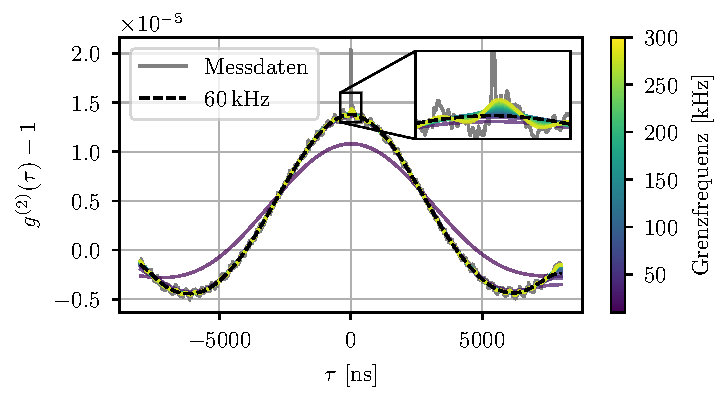
\includegraphics{images/Analysis/lf_offset.pdf}
    \caption{Gezeigt ist ein Vergleich der extrahierten Muster für verschiedene Grenzfrequenzen. In Grau ist die gemittelte $g^{(2)}$-Funktion, aufgenommen mit der Kabelkombination Airborne 5 $40\times 40$ Meter, dargestellt. Farbig hinterlegt sind die ermittelten Muster für verschiedene Grenzfrequenzen. Es ist offensichtlich, dass bei niedrigen Grenzfrequenzen Muster entstehen, die das Störsignal nicht voll erfassen (lila), und bei hohen Grenzfrequenzen (gelb) Muster entstehen, welche Amplitude vom Bunching Peak abschneiden. Eine gute Grenzfrequenz, die das Störsignal großflächig abdeckt und gleichzeitig keine feine Struktur erfasst, liegt bei 60\,kHz und ist schwarz gestrichelt eingezeichnet.}
    \label{fig:lf_offset für verschiedene Grenzfrequenz}
\end{figure}
In der Abbildung ist ersichtlich, dass sowohl zu niedrige als auch zu hoch gewählte Grenzfrequenzen problematisch sind. 
Zu niedrig gewählte Grenzfrequenzen sorgen dafür, dass das Störsignal nicht vollständig erfasst wird (vgl. lila Kurve in \autoref{fig:lf_offset für verschiedene Grenzfrequenz}). 
Je niedriger die Frequenz wird, desto mehr wird statt des gesamten Signals nur dessen Mittelwert extrahiert. 
Eine Subtraktion dieses Musters würde dann dazu führen, dass das Störsignal noch immer vorliegt und lediglich eine geringere Amplitude aufweist. 
Wählt man allerdings die Grenzfrequenz zu hoch, so werden Teile des höherfrequenten Signals der $g^{(2)}$-Funktion fälschlicherweise als Störsignal erkannt. 
Im Extremfall wird so ein Teil des Bunching Peaks bei der Subtraktion abgezogen, was das Ergebnis für $\tau_c$ verfälschen würde. 
Dies ist in \autoref{fig:lf_offset für verschiedene Grenzfrequenz} gelb eingezeichnet. \\
Es gilt also eine Grenzfrequenz zu finden, welche das Störsignal zwar großflächig vollständig erfasst, aber möglichst keinen Einfluss auf die Feinstruktur der Korrelationsfunktion hat. 
Diese Frequenz wird zu etwa 60\,kHz bestimmt. 
Zur Veranschaulichung ist das mit einer Grenzfrequenz von 60\,kHz ermittelte Muster schwarz gestrichelt in \autoref{fig:lf_offset für verschiedene Grenzfrequenz} eingezeichnet. \\

Nach dem Berechnen des Musters wird dieses von der $g^{(2)}$-Funktion abgezogen. 
Durch dieses Vorgehen, erhält man die Korrelationsfunktion, welche in \autoref{fig:g2-offset} dargestellt ist.
\begin{figure}[h]
    \centering
    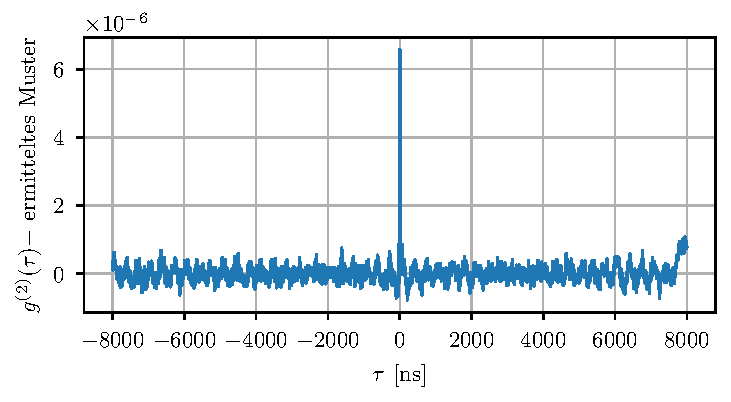
\includegraphics{images/Analysis/g2-lf_offset.pdf}
    \caption{Hier ist dargestellt, wie die $g^{(2)}$-Funktion nach Subtraktion des ermittleten niederfrequenten Störmusters aussieht. Der Bunching Peak sticht nun sehr klar aus dem Hintergrund heraus, welcher um den Wert 0 schwankt.}
    \label{fig:g2-offset}
\end{figure}
Es ist ersichtlich, dass die beschriebene Methode den niederfrequenten Offset im Signal gut entfernt. 
Ein weiterer Vorteil dieser Methode ist, dass der Hintergrund nun um den Wert 0 schwankt, sodass ein Offset in y-Richtung für die spätere Integration (und den Fit) nicht berücksichtigt werden muss. \\
Allerdings soll hier auch auf die Limitationen des erwähnten Vorgehens hingewiesen werden. 
Erstens ist auffällig, dass $g^{(2)}(\tau)$ für $|\tau|\gtrsim 6000\,\mathrm{ns}$ von der Schwankung um 0 abweicht und stattdessen wieder größer wird. 
Dies liegt daran, dass der Tiefpass diese Randregionen aufgrund des abgeschnittenen Signals nicht mehr gut erfassen kann. 
Tatsächlich ist auch schon in \autoref{fig:lf_offset für verschiedene Grenzfrequenz} ersichtlich, dass das extrahierte Muster in den Randregionen stets zu niedrig ist und daher nach der Subtraktion zu hohe Werte liefert. 
Da der Bunching Peak aber für alle verwendeten Kabelkombinationen bei $\tau\approx 0$ liegt, ist die Auswirkung dieser Randbereiche auf $\tau_c$ vernachlässigbar. 
Trotzdem wird für alle folgenden Analyseabschnitte der Definitionsberiech der Offset-korrigierten $g^{(2)}$-Funktion auf $\tau\in[-6000,6000]\,\mathrm{ns}$ eingeschränkt, um einen Einfluss dieser Randeffekte (besonders auf den Fehler auf $\tau_c$, vgl. \autoref{ssec:Fehler von tau_c}) vermeiden zu können. 
Von größerem Belang ist allerdings die Wahl der Grenzfrequenz selbst. 
Wie oben beschrieben erfolgte diese hier anhand von visuellen Überlegungen anhand der $g^{(2)}$-Funktion und dem ermittelten Muster. 
Da sich aber für verschiedene Grenzfrequenzen leicht andere Werte des Musters bei $\tau\approx 0$ ergeben, wirken sich diese auch auf das Integral aus. 
Durch das Festlegen der Grenzfrequenz per Auge ergibt sich ein relativ großer Wertebereich an möglichen Grenzfrequenzen, welche alle ähnlich plausibel erscheinen. 
Die hier gewählten 60\,kHz stellen so etwa die Mitte eines $\pm20\,\mathrm{kHz}$ breiten Bereichs dar. 
Der geschätzte systematische Fehler auf das Integral anhand der später entwickelten Integrationsstrategie liegt im niedrigen einstelligen Bereich. \\

Da dies, wie später klar wird, in der Größenordnung des statistischen Fehlers auf $\tau_c$ liegt, soll an dieser Stelle bereits auf die Notwendigkeit verwiesen werden, für weitere Labormessungen eine tiefergehende Untersuchung bezüglich der Wahl der Grenzfrequenz anzustellen. 
Diese sollte zum Ziel haben, eine besser gerechtfertigte Wahl für die Grenzfrequenz treffen zu können und den systematischen Fehler, der durch die Festlegung dieser Frequenz entsteht, besser zu quantifizieren. 
Da diese Untersuchungen allerdings den Rahmen dieser Arbeit überschreiten würden, wird im Folgenden von einer festen Grenzfrequenz von 60\,kHz ausgegangen, welche, wie in \autoref{fig:g2-offset} zu sehen, bereits zu guten Ergebnissen führt. 

\subsection{Fitfunktion}
\label{ssec:Fitfunktion}    
Nachdem der Offset der Korrelationsfunktion nun abgezogen ist, kann an das Integrieren dieser gedacht werden. 
Dafür sollen in einem späteren Abschnitt verschiedene Integrationsmethoden und Integrationsbereiche miteinander verglichen werden, darunter auch die Integration eines Fits. 
Für diesen späteren Abschnitt ist es also nötig, eine Funktion zu finden, welche den Bunching Peak treffend beschreibt. 
Dies soll das Ziel des jetzigen Abschnittes sein. 

\subsubsection{Bisherige Herangehensweise: Korrelierte gemittelte PMT-Pulse und Gaußfunktion}
\label{sssec:Fitfunktion - Bisherige Herangehensweise}
In der Arbeitsgruppe existieren verschiedene Ideen darüber, welche Fitfunktionen geeingnet sind. 
So wurden für die ersten Labormessungen z. B. gemessene gemittelte Photonenpulse, die während der Ratenkalibration aufgenommen werden (vgl. \autoref{ssec:Datenaufnahme und Waveforms}), korreliert, linear interpoliert und an die Daten gefittet \cite{zmijaOpticalIntensityInterferometry2021}. 
Dies ergibt Sinn, da sich die Ausgangspulse der PMTs (wie in \autoref{ssec:Datenaufnahme und Waveforms} beschrieben) über einige Bins erstrecken und so das zeitlich sehr schmale Bunching Signal verwaschen. 
Die Erwartung an den Bunching Peak in den korrelierten Daten ist daher, dass er sich wie die PMT-Pulse über einige Bins erstreckt und etwa der Form der korrelierten mittleren Pulsform entspricht. \\
Eine weitere Herangehensweise liegt im Fit einer Gaußfunktion an das Signal. 
Dies entspricht der momentanen Herangehensweise der Arbeitsgruppe und wurde z. B. für die Auswertung der Daten der H.E.S.S. Kampagne von 2022 verwendet \cite{zmijaFirstIntensityInterferometry2023}. 
Vorteil dieser Methode ist die relativ einfache, analytische Funktion, welche an die Daten gefittet wird. 
Während bei der vorherigen Methode Daten korreliert und dann interpoliert werden müssen, um die Interpolationsfunktion daraufhin numerisch zu integrieren, kann für die Integration einer Gaußfunktion auf eine simple Formel zurückgegriffen werden:
\todo{cite}
\begin{equation}
    \tau_c^{\mathrm{meas}} = \sqrt{2\pi} a\sigma
\end{equation}
Hierbei sind $a$ die Amplitude und $\sigma$ die Breite der gefitteten Gaußfunktion. 
Dieses Vorgehen vereinfacht den Fit und erlaubt es, relativ einfach Fitparameter wie den Mittlelwert und die Breite $\sigma$ festzuhalten, was aufgrund niedriger Statistik z. B. für die Daten von 2022 nötig war \cite{zmijaFirstIntensityInterferometry2023}. 
Allerdings hat diese Methode auch einen Nachteil, welcher in \autoref{fig:g2-fit Gauß} visualisiert ist. 
\begin{figure}[h]
    \centering
    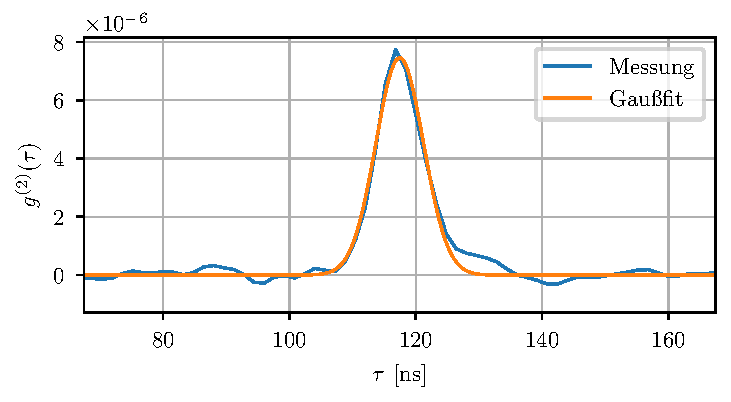
\includegraphics{images/Analysis/g2_gaussfit.pdf}
    \caption{Gezeigt sind die $g^{(2)}$-Funktion für die Messung mit 10\,m und 40\,m Kabeln des Typs Airborne 5. Zusätzlich ist der Fit einer Gaußfunktion eingezeichnet.}
    \label{fig:g2-fit Gauß}
\end{figure}
Durch die Verwendung verschiedener Kabellängen und damit unterschiedlicher Dispersion des Signals für jeden Kanal, folgt für den Bunching Peak als Korrelation der beiden Kanäle, dass dieser asymmetrisch ist. 
Diese Asymmetrie kann vom Gaußfit nicht vollständig erfasst werden -- es wird lediglich die mittlere Abweichung des Fits zu den Datenpunkten minimiert. 
Wie in \autoref{fig:g2-fit Gauß} ersichtlich, werden besonders die Randbereiche des Peaks nicht vom Gaußfit erfasst. 
Da benachbarte Bins allerdings Korrelationen aufweisen und der Bunching Peak über mehrere Bins ausgedehnt ist, enthalten auch die Randbereiche des Peaks das Signal korrelierter Photonen. 
In der vorliegenden Arbeit soll daher, gerade weil es die höhere Statistik der Labormessungen zulässt, von ersterer Methode ausgegangen werden. 
Die Schritte bis zur fertigen Fitfunktion werden im Folgenden erläutert.

\subsubsection{Neue Herangehensweise: Faltung beider Funktionen}
\label{sssec:Fitfunktion - Meine Herangehensweise}
Wie bereits angesprochen verändert sich die Form der Pulse, abhängig von der Kabellänge, die diese durchlaufen. 
In \autoref{fig:mittlere Pulsform} sind zur Veranschaulichung zwei mittlere PMT-Pulse nach Durchlauf eines 40 bzw. 10\,m langen Airborne 5 Kabels dargestellt. 
Diese werden, wie in \autoref{ssec:Datenaufnahme und Waveforms} erwähnt, von der Aufnahmesoftware automatisch gespeichert. 
\begin{figure}[h]
    \centering
    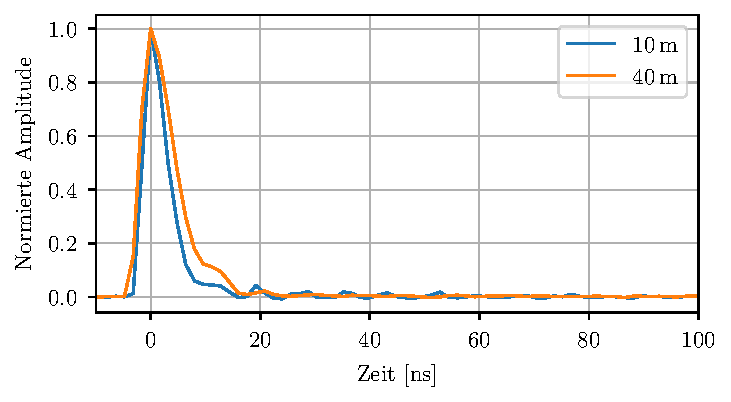
\includegraphics{images/Analysis/mean_pulseshapes.pdf}
    \caption{Gezeigt sind Ausschnitte der mittleren Pulsform bei Verwendung eines 40\,m bzw. 10\,m Airborne 5 Kabels. Es ist erkennbar, dass der orangene Puls breiter als der blaue ist, was an der erhöhten Dispersion im längeren Kabel liegt. Weiterhin wird eine stärkere Dämpfung, d. h. eine Abnahme der Amplitude für längere Kabel, erwartet, was hier aber aufgrund der Normierung nicht direkt sichtbar ist.}
    \label{fig:mittlere Pulsform}
\end{figure}
Wie erwartet, ist der Puls durch das längere Kabel sichtbar verbreitert. 
Im Anschluss werden die beiden mittleren Pulse miteinander korreliert (vgl. \autoref{eq:korrelation}), wobei darauf geachtet wird, dass bei kombinierten Daten von mehreren Messungen auch die aufgenommenen Pulse vor der Korrelation gemittelt werden. 
Zur besseren Interpretation der Parameter in der späteren Funktion wird der so erhaltene Vektor an Datenpunkten zusätzlich normiert, indem durch sein Maximum geteilt wird und so in der Zeit verschoben, dass das Maximum bei $\tau=0$ liegt. 
Da bisher noch keine Funktion, sondern lediglich Datenpunkte vorliegen, wird anschließend eine lineare Interpolation durchgeführt, um die Funktion $y(\tau)$ zu erhalten. 
Diese ist zusammen mit den Datenpunkten der korrelierten Pulsform in \autoref{fig:Interpolation} gezeigt. 
\begin{figure}[h]
    \centering
    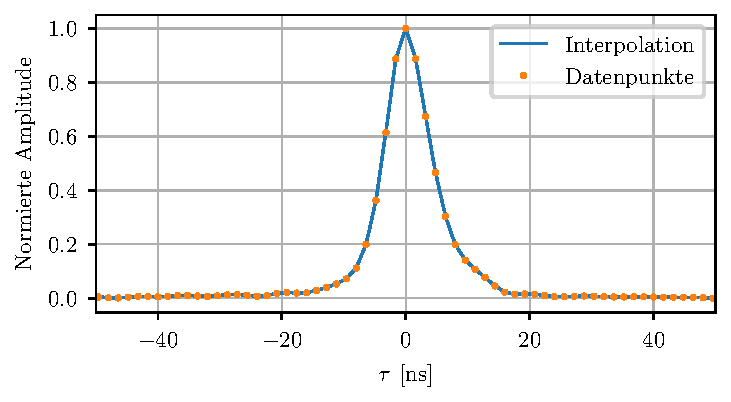
\includegraphics{images/Analysis/interpolation.pdf}
    \caption{Dargestellt ist das Ergebnis der diskreten Korrelation (orange) und die lineare Interpolation davon (blau).}
    \label{fig:Interpolation}
\end{figure}
Die so ermittelte Funktion $y(\tau)$ kann nun durch freie Parameter ergänzt werden, sodass diese an die Datenpunkte der $g^{(2)}$-Funktion gefittet werden kann. 
Notwendig sind ein Offset in x-Richtung $\tau_0$ und ein Amplitudenfaktor $a$, welcher den Fit in y-Richtung staucht und streckt. 
Weiterhin kann eine Streckung des Peaks in x-Richtung im Vergleich zu $y(\tau)$ vorliegen, was auf eine Veränderung in der Zeitauflösung der Messung im Vergleich zur Kalibration zurückzuführen ist. 
Da für die Konstruktion der korrelierten mittleren Photonenpulse Photonenpeaks der Raten-Kalibrationsmessung zuerst übereinander verschoben und anschließend gemittelt werden, enthält $y$ bereits die Zeitauflösung des Systems, welches durch das Binning bedingt ist. 
Eine zusätzliche Verbreiterung des Bunching Peaks im Vergleich zu $y(\tau)$ wäre daher auf eine zusätzliche statistische Schwankung der Position des Bunching Peaks zurückzuführen, welche in der Kalibrationsmessung nicht vorliegt. 
Beispiele hierfür sind zeitliche Schwankungen der PMT-Ausgangssignale oder eine durch das Teleskop selbst bedingte Verschlechterung der Zeitauflösung (vgl. \autoref{ssec:Vergleich mit Hess}).

Um diesen möglichen Effekt in der Fitfunktion zu quantifizieren, wird eine Vorgehensweise ähnlich der in \cite{lasseguesFieldIntensityCorrelations2022} gewählt, bei der die Funktion $y(\tau)$, welche der Theoriefunktion bei idealer Zeitauflösung entspricht, mit einer Gaußfunktion gefalten, welche über ihre Breite $\sigma$ eine zusätzliche Verschlechterung der Zeitauflösung ausdrückt. 
Es folgt:
\begin{equation}
    f(\tau, a, \sigma, \tau_0) = ay(\tau - \tau_0) * \mathrm{e}^{-\frac{\tau^2}{2\sigma^2}}
\end{equation}
Weil die verwendete Routine zur Faltung nur für Vektoren und nicht für Funktionen definiert ist, ergeben sich in der Auswertung noch leichte Abweichungen von dieser Vorgehensweise. 
So werden die linke und rechte Seite der Faltung erst in einem ausreichend großen und fein gewählten Intervall unter Einsetzung der Parameter $a=1$ und $\tau_0 = 0$ ausgewertet, woraufhin die diskrete Faltung der beiden Vektoren durchgeführt wird. 
Um anschließend wieder eine Funktion zu erhalten, welche für alle $\tau$ definiert ist, wird erneut eine lineare Interpolation durchgeführt und normiert, was zu Funktion $h$ führt. 
Schlussendlich ergibt sich die Fitfunktion also zu:
\begin{equation}
    f(\tau, a, \tau_0, \sigma) = ah(\tau- \tau_0, \sigma)
    \label{eq:fit funktion final}
\end{equation} 
Durch die Variation der Parameter während der Fitroutine geht der Parameter $\sigma$ dann vor der Faltung ein, während die $a$ und $\tau_0$ nach der Faltung und Interpolation eingehen. 
Durch die erwähnten Normierungs- und Verschiebungsschritte der Funktionen, welche die Funktion $f$ bilden, entspricht (bis auf für den Fit unwesentliche Abweichungen) $a$ nun der Amplitude des Fits und $\tau_0$ seinem Offset von $\tau=0$. 
Auf diese Weise ist eine Einschränkung der Fitparameter für die spätere Auswertung möglich, was die Konvergenz der Fits verbessert. 
Die Größe von $\sigma$ beschreibt eine mögliche systembedingte Zeitauflösung während der Messung, welche während der Kalibration nicht vorliegt. 
Wie eine Variation des Fitparameters $\sigma$ die resultierende Funktion $f$ beeinflusst, ist in \autoref{fig:Fitfuktion für verschiedene sigma} für $a=1$, $\tau_0=0$ dargestellt. 
\begin{figure}[h]
    \centering
    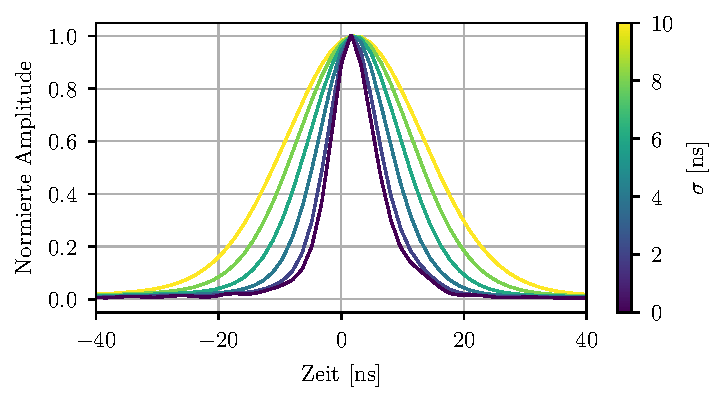
\includegraphics{images/Analysis/corr_pulses_diff_sigma.pdf}
    \caption{Dargestellt ist ein Ausschnitt der resultierenden Fitfunktion $f$ bei Variation des Fitparamters $\sigma$ ($a=1$, $\tau_0=0$). Für sehr niedrige $\sigma$ entspricht die Funktion praktisch der korrelierten Pulsform der PMTs und für größer werdende $\sigma$ nähert sich die Funktion immer mehr der Form einer Gaußfunktion an.}
    \label{fig:Fitfuktion für verschiedene sigma}
\end{figure}
Es ist ersichtlich, dass eine Erhöhung des Parameters $\sigma$ zu einer Verbreiterung der Fitfunktion führt, welche zudem immer glatter und gaußförmiger wird. \\

Die Konstruktion und Verwendung der Fitfunktion, wie oben beschrieben, hat einige Vorteile. 
Wie bereits angesprochen, entspricht eine Faltung von einer Gaußfunktion, welche die Zeitauflösung während der Messung enthält, mit der gemessenen erwarteten Peakform bei bestmöglicher Zeitauflösung am ehesten der theoretischen Erwartung an die Form des Bunching Peaks. 
Zudem werden durch dieses Vorgehen eine mögliche Asymmetrie des Peaks und Ringing der PMTs berücksichtigt, was zu einer genaueren Bestimmung des Integrals und damit der Kohärenzzeit führt. 
Durch die Veränderung der korrelierten Pulsform für jede Kabellängenkombination ändert sich auch die Fitfunktion und bildet so die kabelabhängige Form des Bunching Peaks besser ab. 
Zusätzlich kann durch dieses Vorgehen die Zeitauflösung des Systems aus den gemessenen Daten bestimmt werden. 
Aus diesen Gründen wird im Folgenden auf die soeben beschriebene Fitfunktion zurückgegriffen. 

\subsection{Wahl der Integrationsmethode und Integrationsgrenzen}
\label{ssec:Wahl der Integrationsmethode}
Zur Vollständigkeit soll in diesem Analyseteil kurz darauf eingegangen werden, ob ein Fit an die Daten notwendig ist oder ob es ausreicht, die gemittelte $g^{(2)}$-Funktion direkt zu integrieren. 
Im selben Zuge wird die Wahl der Integrationsgrenzen für die spätere Analyse motiviert. 
Hierfür wird exemplarisch ein Fit von \autoref{eq:fit funktion final} an die gemittelten, Offset-korrigierten Daten der Airborne $10\times 10\,\mathrm{m}$-Messung durchgeführt. 
Anschließend werden sowohl der Fit als auch die Daten selbst numerisch integriert. 
Der Fit erfolgt in einem breiten Intervall von $\pm 100$ Bins, d. h. $\pm 160\,\mathrm{ns}$ um den Peak herum. 
Die Integration erfolgt in einem Intervall $[\tau_{\mathrm{max}}-w, \tau_{\mathrm{max}}+w]$, wobei $\tau_{\mathrm{max}}$ dem Zeitpunkt entspricht, an welchem $g^{(2)}(\tau)$ maximal ist und die Integrationsbreite $w$ im Bereich $w\in [1,160]\,\mathrm{ns}$ variiert wird. 
Das Resultat dieser Analyse ist in \autoref{fig:integration verschiedene Breiten} dargestellt. 
\begin{figure}[hp]
    \centering
    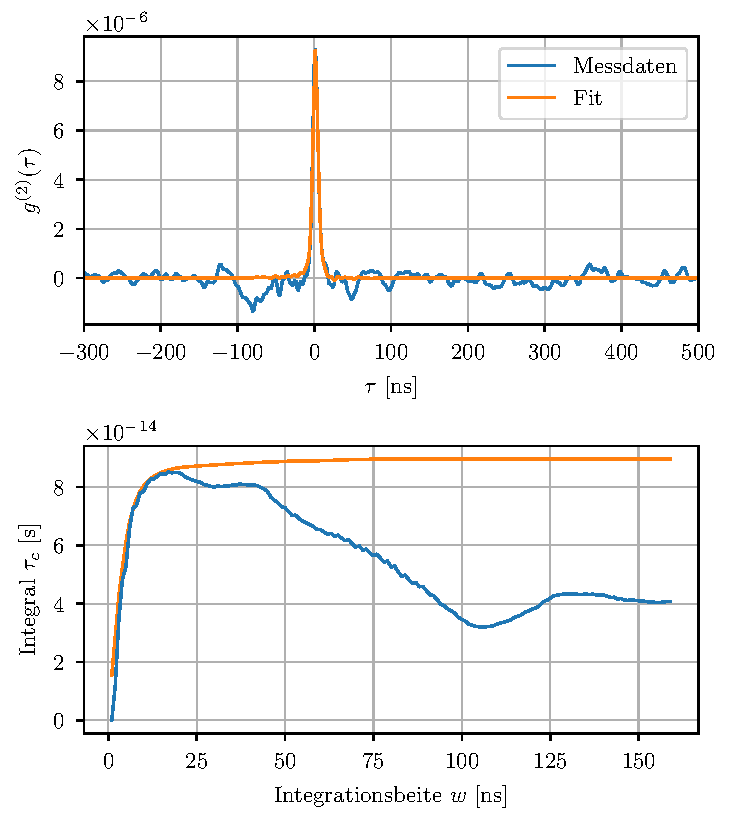
\includegraphics{images/Analysis/integration_different_width.pdf}
    \caption{Oben ist die $g^{(2)}$-Funktion (blau) sowie ein Fit an diese (orange) zu sehen. Für verschiedene Integrationsbreiten ist unten in gleichen Farben abgebildet, wie sich die resultierenden Integrale der beiden Funktionen entwickeln. Für die Integration der Rohdaten ist eine deutliche Fluktuation des Integrals zu sehen, während die Integration des Fits sich auch für große Breiten stabil verhält.}
    \label{fig:integration verschiedene Breiten}
\end{figure}
In der Grafik ist erkennbar, dass die Integration des Fits für steigende Integrationsbreiten zunimmt und schließlich einen stabilen Wert annimmt. 
Dies ergibt Sinn, da die Interpolation der Daten im letzten Schritt der Konstruktion der Fitfunktion außerhalb des Bereichs der Datenpunkte den konstanten Wert 0 annimmt. 
Da weiterhin kein y-Offset gefittet wird, ändert sich das Integral ab einer gewissen Integrationsbreite daher nicht mehr. 
Die direkte Integration der Messdaten hingegen ist stark abhängig von Fluktuationen der Korrelationsfunktion außerhalb des Bunching Peaks. 
So sinkt diese z. B. zwischen $w=50\,\mathrm{ns}$ und $w=100\,\mathrm{ns}$ stark, was an dem zufällig niedrigen Wert der Korrelationsfunktion links vom Bunching Peak (vgl. \autoref{fig:integration verschiedene Breiten} oben) liegt. \\

Da ein Ziel dieser Arbeit sein soll, Integrale verschiedener Kabellängen miteinander zu vergleichen und es keine von vornherein \glqq richtige\grqq\;Wahl der Integrationsbreite gibt, welche nur Signal und kein Rauschen erfasst, ist Stabilität im Wert von $\tau_c$ für verschiedene Integrationsbreiten essentiell. 
Da benachbarte Bins wie erwähnt korreliert sind, sind häufig breite Fluktuationen von $g^{(2)}(\tau)$ nach unten oder oben anzutreffen, welche die Differenz zwischen Integralen für eine beliebige Integrationsbreite stark beeinflusst. 
Aus dem Grund der besseren Vergleichbarkeit der Messreihen untereinander wird daher die Methode gewählt, einen Fit von \autoref{eq:fit funktion final} an die Daten durchzuführen und diesen anschließend zu integrieren. 
Aus erwähnter Konstruktion mittels Interpolation und aus \autoref{fig:integration verschiedene Breiten} unten wird weiterhin ersichtlich, dass sich das Integral lediglich bis $w\approx 100\,\mathrm{ns}$ nennenswert ändert. 
Als Integrationsbreite ist also ein Wert von $w\gtrsim 100\,\mathrm{ns}$ geeignet, wobei ein zu großer Intervall per Konstruktion wie erwähnt keine Probleme verursacht. 
Aus diesem Grund wird die Funktion $f(\tau, a, \tau_0, \sigma)$ für die folgende Analyse stets in einem Intervall von $\pm 100$ Bins bzw. $\pm 160\,\mathrm{ns}$ gefittet und integriert. 

\subsection{Fehler von \texorpdfstring{$\tau_c$}{tc}}
\label{ssec:Fehler von tau_c}
Nachdem im vorigen Abschnitt auf das Integrieren des Bunching Peaks eingegangen wurde, soll im Folgenden der Fehler ebendieses Integrals abgeschätzt werden. 
Durch die Korrelation benachbarter Bins lässt sich nicht ohne weiteres ein Fehler auf den Wert der Korrelationsfunktion bestimmen, welcher durch den Fit fortgepflanzt werden kann, da die verwendete $\chi^2$-Minimierung statistisch unabhängige Fehler zwischen Samples voraussetzt \cite{vugrinConfidenceRegionEstimation2007}. 
Stattdessen wird eine andere Methode genutzt, welche das Rauschen der $g^{(2)}$-Funktion unmittelbar mit einbezieht. 
Dafür wird zuerst wie im letzten Abschnitt beschrieben ein Fit an den Bunching Peak durchgeführt, welcher daraufhin integriert wird, um den Wert für $\tau_c$ zu erhalten. 
Um anschließend auf den Fehler zu schließen, wird ebendieser Fit in feinen Schritten über die $g^{(2)}$-Funktion verschoben und zu dieser an der jeweiligen Stelle addiert. 
Es wird der Fit an die Daten, statt der Bunching Peak selbst, verschoben, um lediglich das Signal, nicht aber das umliegende Rauschen mitzuverschieben, welches einen systematischen Einfluss auf den Verlauf des Rauschens um den verschobenen Peak hätte. 
Der so erhaltene Peak entspricht jenem, der gemessen worden wäre, wenn das Rauschen um den Peak zufällig anders verschoben wäre. 
Da der hauptsächliche Fehler auf das Integral der zufälligen Position des Peaks in der $g^{(2)}$-Baseline entspricht (im Besonderen, ob der Peak auf einer niedrigen oder hohen Fluktuation liegt), lässt sich durch die Änderung des Integrals bei verschiedener Peakposition der Fehler auf das Integral gut abschätzen. 
Für jede Peakposition wird anschließend erneut mit derselben Methodik gefittet und integriert. 
Das Resultat dieses Vorgehens ist eine Liste an Integralen. 
Für den Fehler auf das Integral wird abschließend die Standardabweichung dieser Liste bestimmt, um zu quantifizieren, wie stark die Integrale im Mittel unter dem Einfluss des Rauschens in der Baseline schwanken. 
Die Standardabweichung als Maß für den Fehler zu wählen, ergibt an dieser Stelle Sinn, da die Schwankung der Baseline als näherungsweise gaußverteilt angenommen werden kann. 
Dies liegt daran, dass die Wahrscheinlichkeitsverteilung der Intensitätsfluktuationen einer chaotischen Lichtquelle für $\tau\gg \tau_c$ der Poissonverteilung des kohärenten Lichts um $g^{(2)}=1$ entspricht, was für hohe Photonenzahlen in eine Gaußverteilung übergeht \cite[Kap. 5.5]{foxQuantumOpticsIntroduction2006}.
Obwohl diese Fluktuationen sich in der Theorie exakt kürzen (vgl. \autoref{eq:g2_final}), sodass $g^{(2)}(\tau \gg \tau_c) = 1$, ist dies im Experiment aufgrund der Unterteilung in Zeitbins, Messabschnitte und weiterer Effekte nicht der Fall, sodass eine gaußverteilte Schwankung um die 1 verbleibt. \todo{macht das sinn?} \\

Exemplarisch ist das oben erklärte Vorgehen für die $10\times 10\,\mathrm{m}$-Airborne 5 Messung in \autoref{fig:Fehler auf tc} gezeigt. 
\begin{figure}[hp]
    \centering
    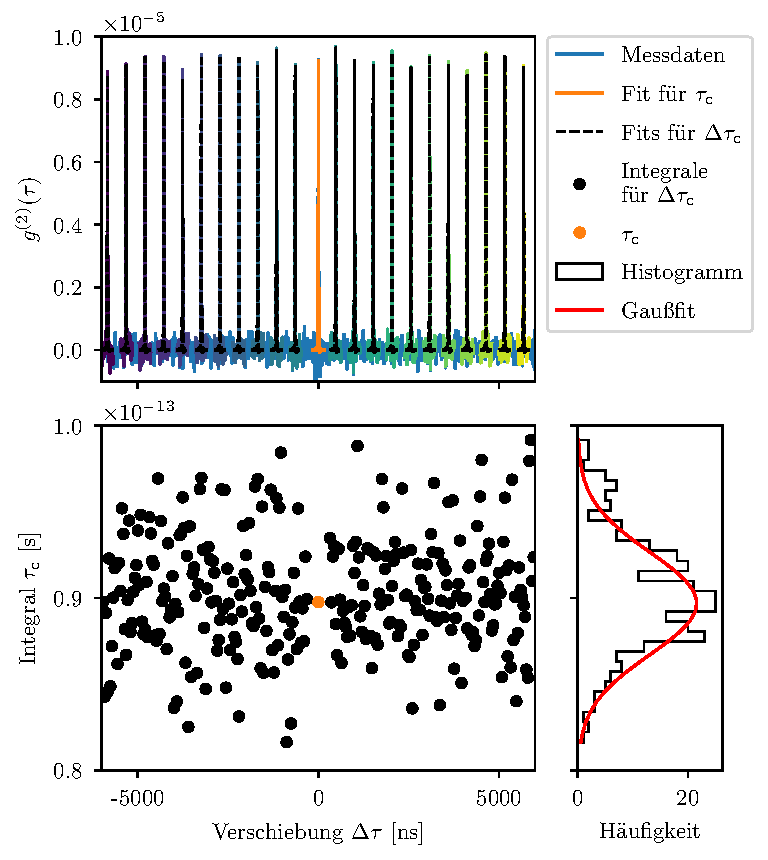
\includegraphics{images/Analysis/integration_error.pdf}
    \caption{Oben sind die gemittelte $g^{(2)}$-Funktion (blau), der Fit des Bunching Peaks (orange), die verschobenen und zur Baseline addierten Peaks (Farbgradient lila-gelb, je nach Verschiebung) und die erneut durchgeführten Fits an diese (schwarz gestrichelt) dargestellt. Unten links sind die reultierenden Integrale der verschobenen Fits und des Fits an den Bunching Peak (entspricht der Verschiebung $\Delta\tau=0$) im selben Farbschema dargestellt. Zur Bestimmung des Fehlers $\sigma_{\tau_c}$ wird die Standardabweichung der Verteilung der schwarzen Punkte berechnet, während $\tau_c$ dem orangenen Punkt entspricht. Unten rechts ist abschließend die Verteilung der schwarzen Punkte histogrammiert. Weiterhin ist ein Gaußfit (rot) durchgeführt worden, dessen Verlauf die Erwartung bestätigt, dass die Verteilung der Integrale gaußverteilt ist.}
    \label{fig:Fehler auf tc}
\end{figure}
Zuerst erfolgt im obigen Graph der Fit und die Integration des Bunching Peaks. 
Für alle Fits wurden erneut Fit- und Integrationsfenster von $\pm 100$ Bins gewählt (vgl. \autoref{ssec:Wahl der Integrationsmethode}). 
Anschließend wird die Fitfunktion in $25\,ns$-Schritten zwischen $\tau = -6000\,\mathrm{ns}$ und $\tau = 6000\,\mathrm{ns}$ verschoben, wobei darauf geachtet wird, die Region des ursprünglichen Bunching Peaks auszulassen. 
Der verschobene Peak wird auf die $g^{(2)}$-Baseline addiert, was im angesprochenen Graph als Farbverlauf (der Übersichtlichkeit wegen nur für wenige Verschiebungen) eingezeichnet ist. 
Für jede Verschiebung wird erneut ein Fit durchgeführt und integriert, was im unteren linken Teil der \autoref{fig:Fehler auf tc} als schwarzer Punkt aufgetragen ist. 
Wird nun die Standardabweichung der schwarzen Punkte (d. h. der Integrale für verschiedene Verschiebungen) gebildet, lässt sich damit wie oben beschrieben der Fehler auf $\tau_c$ bestimmen. 
Zur Verifikation der Annahme einer Gaußvertielung der Integrale, die in die Berechnung des Fehlers mit eingeht, ist unten links zudem ein Histogramm der angenommenen Integralwerte gegeben. 
An dieses wurde ein Fit einer Gaußfunktion durchgeführt, welche in guter Übereinstimmung mit der Verteilung der Punkte ist. 
Wie anhand theoretischer Überlegungen erwartet, ist eine Gaußverteilung also eine gerechtfertigte Annahme an die Verteilung der Änderung der Integrale mit verschiedenem $\Delta\tau$. 
Dies bestätigt, dass die gewählte Methode, insbesondere die Berechnung der Standardabweichung, geeignet ist, um die Schwankung der Integrale und daher $\sigma_{\tau_c}$ zu quantifizieren. 

\subsection{Ergebnisse für verschiedene Kabelkombinationen}
\label{ssec:Ergebnisse für verschiedene Kabelkombinationen}
Die in den obigen Abschnitten angesprochenen Verfahren zum Fit, zur Integration und zur Bestimmung des Fehlers auf $\tau_c$ werden im Folgenden auf die gemessenen Daten angewandt. 
Daten wurden insgesamt mit fünf Kabelkombinationen aufgenommen. 
Wie bereits erwähnt werden je 10{.}000 Dateien gemittelt, was nach \autoref{ssec:mittelung und filter} etwa 9{,}5\,h reiner Messdauer entspricht. 
Verwendete Kabellängenkombinationen sind $10\times 10\,\mathrm{m}$ und $10\times 40\,\mathrm{m}$ für jeweils Airborne 5 und LMR 400 sowie eine Messung bei $40\times 40\,\mathrm{m}$, welche lediglich für die Kabel des Typs Airborne 5 durchgeführt wurden. 
Letztere Messung konnte aufgrund eines fehlenden zweiten LMR 400 Kabels mit Länge 40\,m und mangelnder Zeit für die Bestellung nicht mehr durchgeführt werden. 
Die gemittelten, Offset-korrigierten $g^{(2)}$-Funktionen, Fits daran, sowie die resultierenden Integrale und Fehler sind in \autoref{fig:integrale ergebnisse} dargestellt. 
Die exakten Werte der bestimmten Kohärenzzeiten sind zudem in \autoref{tab:gemessene Kohärenzzeiten} aufgelistet. 
\begin{figure}[hp]
    \centering
    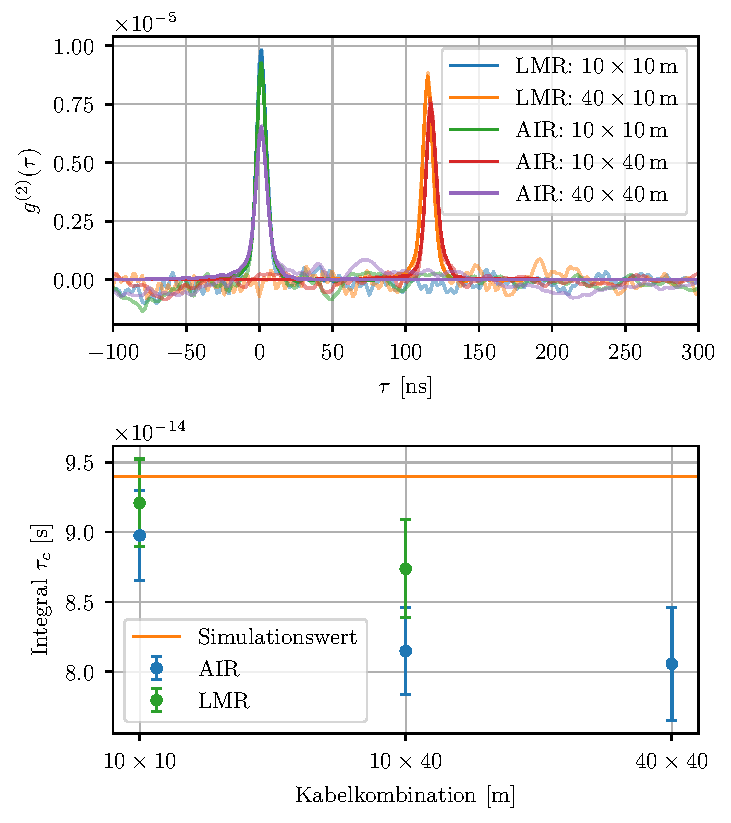
\includegraphics{images/Analysis/all_combined.pdf}
    \caption{Dargestellt sind oben die gemittelten $g^{(2)}$-Funktionen und Fits und unten die resultierenden Integrale und Fehler für alle verwendeten Kabelkombinationen.}
    \label{fig:integrale ergebnisse}
\end{figure}
Im obigen Graph ist qualitativ erneut erkennbar, dass die Peaks eine geringere Amplitude aufweisen, je länger die kombinierte Kabellänge ist. 
Dies deckt sich mit bisherigen Resultaten von H.E.S.S. \cite{zmijaFirstIntensityInterferometry2023}. 
Weiterhin auffällig ist, dass der Peak für ungleiche Kabellängen von der Null verschoben ist. 
Dies stimmt mit der Erwartung überein, da das Signal eines Kanals vor der Korrelation eine um die Kabellängendifferenz erhöhte Strecke durchläuft. 
Unter Berücksichtigung der Ausbreitungsgeschwindigkeiten im Kabel von 84 bzw. 87\% der Lichtgeschwindigkeit für Airborne 5 bzw. LMR 400 \cite{s.r.lAirborne10Coaxial,LMR400CoaxCable} erklärt sich so die gemessene Verschiebung um etwa 115\,ns. 
Im unteren Teil der \autoref{fig:integrale ergebnisse} ist zu sehen, wie sich die Integrale bei gegebener Kabelkombination verhalten. 
Der berechnete Wert der Integrale nimmt mit steigender Dämpfung der verwendeten Kabel ab. 
So weisen kürzere Kabelkombinationen längere und längere Kombinationen kürzere Kohärenzzeiten auf. 
Weiterhin sind die Integrale der LMR-Kabel, welche eine geringere Dämpfung des Signals aufweisen, stets höher als die der Airborne-Kabel. 
Durch Betrachten des als horizontale Linie eingezeichneten, in \autoref{sec:Aufbau} bestimmten Erwartungswerts an die Kohärenzzeit wird dies nochmals verdeutlicht. 
Es scheint, als würde eine Kombination idealer $0\times 0\,\mathrm{m}$ langer Kabel eine Kohärenzzeit ergeben, welche sich gut mit der Simulation deckt. \\
Allerdings muss mit obiger Interpretation vorsichtig umgegangen werden. 
Es ist zu betonen, dass diese Ergebnisse lediglich ein Indiz für die erwähnte Abhängigkeit der Kohärenzzeit von der Kabeldämpfung darstellen. 
Betrachtet man die eingezeichneten Fehlerbalken, welche aufgrund der Überlegungen in \autoref{ssec:Fehler von tau_c} 1-$\sigma$-Intervallen entsprechen, ist festzustellen, dass die Unterschiede der Integrale nicht statistisch signifikant sind. 
Besonders zwischen den Datenpunkten $10\times 40\,\mathrm{m}$ und $40\times 40\,\mathrm{m}$ ist im Rahmen der Unsicherheit kein Unterschied festzustellen. 
Auch wenn sich die Fehlerbalken der erwähnten Messungen nicht mit der $10\times 10\,\mathrm{m}$-Messung decken, ist dies nicht automatisch auf einen Unterschied von $\tau_c$ zurückzuführen. 
Schließlich ist die Bedeutung der Fehlerbalken vielmehr, dass jeder aufgetragene Punkt bei einer Wiederholung der Messung in etwa 32\% der Fälle außerhalb der Fehlerbalken liegt. 
Zusammenfassend lässt sich also kein statistisch signifikanter Einfluss der Kabellänge bzw. Dämpfung der Kabel auf den Wert von $\tau_c$ feststellen. 
Allerdings bleibt zu erwähnen, dass sich die Abnahme der Integralwerte für steigende kombinierte Kabellänge in allen von der Arbeitsgruppe bisher durchgeführten Experimenten zeigt. \todo{Cite personbal correspondance?}
Auch wenn die vorgestellten Ergebnisse dies nicht einwandfrei beweisen können, gibt es daher deutliche Indize für einen bisher unbekannten Einfluss. 
Langzeitmessungen mit höherer Statistik sind vonnöten, um statistisch aussagekräftigere Ergebnisse zu erhalten. 
Mit diesen ließe sich besser verstehen, ob es einen Effekt gibt -- wenn ja, woher dieser genau kommt und an welchem Punkt der Signalverarbeitung er sich auswirkt. 
Während, wie in \autoref{ssec:Intensitätsinterferometrie} beschrieben, ein direkter Einfluss einer zeitunabhängigen Dämpfung auf $g^{(2)}$ theoretisch nicht zu erwarten ist, ist z. B. eine Dämpfungsabhängigkeit an einem einzelnen Schritt im komplizierten Pre-Processing der Daten durchaus nicht auszuschließen und bedarf weiterer Untersuchung mit statistisch aussagekräftigeren Daten. 

\begin{table}[h]
    \centering
    \begin{tabular}{|c|c|c|} \hline
        Kabeltyp    & Kabellänge [m] & Kohärenzzeit [fs]  \\\hline
        LMR 400     & $10\times 10$  & $92{,}1 \pm 3{,}1$ \\\hline
        LMR 400     & $10\times 40$  & $87{,}4 \pm 3{,}5$ \\\hline
        Airborne 5  & $10\times 10$  & $89{,}8 \pm 3{,}2$ \\\hline
        Airborne 5  & $10\times 40$  & $81{,}5 \pm 3{,}1$ \\\hline
        Airborne 5  & $40\times 40$  & $80{,}6 \pm 4{,}0$ \\\hline
    \end{tabular}
    \caption{Aufgelistet sind die bestimmten Kohärenzzeiten und Fehler für die verwendeten Kabelkombinationen. Die theoretische Erwartung liegt bei $\tau_c^{\mathrm{meas}}=94\,\mathrm{fs}$, vgl. \autoref{sec:Aufbau}}.
    \label{tab:gemessene Kohärenzzeiten}
\end{table}
Aus den Fits lassen sich weiterhin Werte für die Parameter $\sigma$ extrahieren welche, wie in \autoref{ssec:Fitfunktion} beschrieben, eine zusätzliche Verbreiterung des Bunching Peaks im Vergleich zur Kalibrationsmessung beschreiben. 
Die Ergebnisse, die sich aus den durchgeführten Fits für den Parameter $\sigma$ ergeben, liegen in etwa im Bereich von $0{,}05\,ns$ bis $0{,}8\,\mathrm{ns}$. 
Betrachtet man hierzu \autoref{fig:Fitfuktion für verschiedene sigma}, fällt auf, dass die resultierende Fitfunktion bei solch kleinen $\sigma$ praktisch den korrelierten mittleren Pulsen entspricht, die Faltung in diesem Fall also praktisch keinen Einfluss hat. 
Aus diesem Grund ist es der Fitroutine für die in \autoref{fig:integrale ergebnisse} dargestellten Fits auch nicht möglich, den Fehler auf $\sigma$ abzuschätzen, weshalb die oben genannten Werte für $\sigma$ nicht als tatsächliche Resultate zu interpretieren sind. 
Stattdessen sollte aus diesen der Schluss gezogen werden, dass es keine nennenswerten Einflüsse während der Messung gibt, die zu einer Verbreiterung des Bunching Peaks führen und zur Kalibration noch nicht vorliegen. 
Für Labormessungen lässt sich also abschließend festhalten, dass die Faltung mit einer Gaußfunktion überflüssig (aber nicht falsch) ist und der Fit der korrelierten PMT-Pulse ausreichend ist. 
Dies ist allerdings keineswegs allgemein gültig, wie im folgenden Abschnitt gezeigt wird.

\subsection{Vergleich mit Daten der H.E.S.S. Kampagne 2022}
\label{ssec:Vergleich mit Hess}
Als Abschluss der Analyse werden die erhaltenen Ergebnisse aus vorigem Abschnitt noch mit den zwischen 19. und 21.4.2022 an den H.E.S.S. Teleskopen gemessenen Daten für Shaula verglichen. 
Dieser Vergleich dient als Indiz dafür, ob sich die gemessenen Unterschiede von $\tau_c$ für verschiedene Kabellängen mit den obig präsentierten Laborergebnissen decken. 
Wäre dies der Fall, würde das darauf hinweisen, dass in beiden Fällen möglicherweise derselbe Effekt vorliegt. 
Die Daten jeder Kabellängenkombination sowie der mittleren Pulsformen werden über die erwähnten drei Nächte zuerst gemittelt und gespeichert. 
Anschließend werden die gemittelten $g^{(2)}$-Funktionen von Shaula mit der oben beschriebenen Methode gefittet und integriert, um möglichst vergleichbare Ergebnisse zu den Labormessungen zu schaffen. 
Die so ermittelten Ergebnisse sind erneut als Graph (\autoref{fig:integration shaula}) sowie tabellarisch (\autoref{tab:Kohärenzzeiten Shaula}) dargestellt. 
\begin{figure}[h]
    \centering
    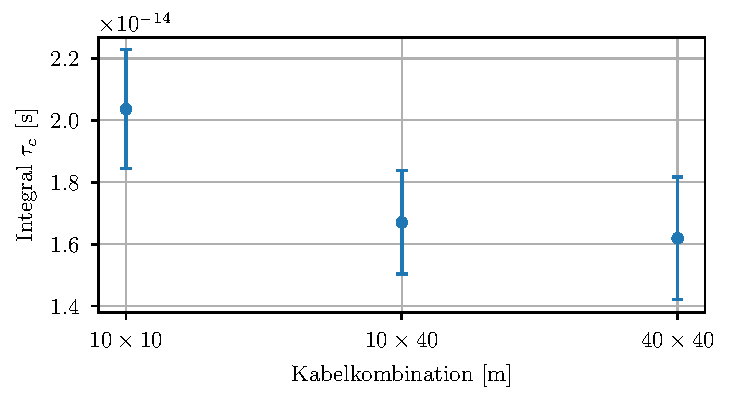
\includegraphics{images/Analysis/shaula_integrals.pdf}
    \caption{Gezeigt sind die berechneten $\tau_c$ die sich bei Integration der Shaula-Daten ergeben.}
    \label{fig:integration shaula}
\end{figure}
\begin{table}[h]
    \centering
    \begin{tabular}{|c|c|c|} \hline
        Kabeltyp    & Kabellänge [m] & Kohärenzzeit [fs]  \\\hline
        Airborne 5  & $10\times 10$  & $20{,}3 \pm 1{,}9$ \\\hline
        Airborne 5  & $10\times 40$  & $16{,}7 \pm 1{,}7$ \\\hline
        Airborne 5  & $40\times 40$  & $16{,}2 \pm 2{,}0$ \\\hline
    \end{tabular}
    \caption{Aufgelistet sind die bestimmten Kohärenzzeiten und Fehler für die verwendeten Kabelkombinationen bei der H.E.S.S.-Messung von Shaula. Für die Messung wurden Kabel des Typs Airborne 5 verwendet \cite{zmijaFirstIntensityInterferometry2023}.}
    \label{tab:Kohärenzzeiten Shaula}
\end{table}
Für einen Vergleich der beiden Messungen bietet es sich an, zu berechnen, um welchen Faktor das Integral des $10\times 40\,\mathrm{m}$-Peaks bzw. des $40\times 40\,\mathrm{m}$-Peaks kleiner ist als das Integral des $10\times 10\,\mathrm{m}$-Peaks, welches für beide Messungen am größten ist. 
Konkret wird also folgendes Verhältnis verglichen, dessen Fehler sich aus gaußscher Fehlerfortpflanzung ergibt:
\begin{equation}
    r_i = \frac{\tau_{c,10\times10}}{\tau_{c,i}} \pm \sqrt{\left(\frac{\sigma_{\tau_{c,10\times10}}}{\tau_{c,i}}\right)^2 + \left(\frac{\tau_{c,10\times10} \cdot \sigma_{\tau_{c,i}}}{\tau_{c,i}^2}\right)^2}
\end{equation}
Hierbei ist $\tau_{c,i}$ die Kohärenzzeit für die $10\times 40\,\mathrm{m}$-Messung bzw. die $40\times 40\,\mathrm{m}$-Messung und $\sigma_{\tau_{c,i}}$ der jeweilige Fehler darauf. 
Als Ergebnis für beide Raten und beide Messungen ergeben sich die in \autoref{tab:labor shalua r} gelisteten Werte. 
\begin{table}[h]
    \centering
    \begin{tabular}{|c|c|c|}\hline
        Kabellänge $i$ [m]       & Ergebnis Labor      & Ergebnis Shaula     \\\hline
        $10\times 40$            & $1{,}10 \pm 0{,}06$ & $1{,}22 \pm 0{,}17$ \\\hline
        $40\times 40$            & $1{,}11 \pm 0{,}07$ & $1{,}26 \pm 0{,}19$ \\\hline
    \end{tabular}
    \caption{Vergleichend dargestellt sind die Ergebnisse für die Raten $r_i$ bei den Labormessungen und Shaula.}
    \label{tab:labor shalua r}
\end{table}
Die Werte für das Labor $L$ und für Shaula $S$ sind innerhalb ihrer Unsicherheit verträglich, wenn die Differenz $S-L$ innerhalb ihres Fehlers $\sqrt{\sigma_L^2 + \sigma_L^2}$ auf Null abfällt. 
Da dies für beide Kabellängenkombinationen gegeben ist, lässt sich folgern, dass die Unterschiede in $\tau_c$ -- sollten sie denn existieren, was aufgrund der großen Fehler nicht als gesichert angenommen werden kann -- für Labormessungen und Messungen an den H.E.S.S.-Teleskopen im  gleichen Rahmen auftreten. 
Es gibt also ein deutliches Indiz dafür, dass bei beiden Aufbauten die Änderung im Integral (sollte sie existieren) durch das gleiche, vom Teleskop unabhängige Phänomen hervorgerufen wird. \\

Aus den Fits an die Shaula-Daten lassen sich zudem die Fitparameter $\sigma$, sowie deren Fehler extrahieren. 
Aufgrund der niedrigeren Zeitauflösung der Teleskope im Vergleich zum Laboraufbau wird erwartet, dass dieser im Bereich einstelliger Nanosekunden liegt. 
Dies liegt daran, dass Photonen, die auf die Spiegel der H.E.S.S.-Teleskope treffen, unterschiedlich lange Wege zurücklegen müssen, bis sie an den PMTs detektiert werden können. 
Daraus folgt eine Verschlechterung der Zeitauflösung im Vergleich zur Kalibrationsmessung, welche, wie in \autoref{ssec:Fitfunktion} angesprochen, zu einem Verwaschen des Bunching Peaks führt, das durch den Parameter $\sigma$ im Fit erfasst wird. 
Aus den Fits ergeben sich die in \autoref{tab:sigma Shaula} dargestellten Werte, aus denen unter Verwendung eines mit dem Einzelfehler der Werte gewichteten Mittelwerts folgt: 
\begin{equation}
    \overline{\sigma} = 2{,}01 \pm 0{,}20\,\mathrm{ns}
\end{equation}
\begin{table}[h]
    \centering
    \begin{tabular}{|c|c|}\hline
        Kabellänge $i$ [m] & Zeitauflösung [ns]  \\\hline
        $10\times 10$      & $2{,}51 \pm 0{,}32$ \\\hline
        $10\times 40$      & $1{,}15 \pm 0{,}44$ \\\hline
        $40\times 10$      & $1{,}71 \pm 0{,}45$ \\\hline
        $40\times 40$      & $2{,}23 \pm 0{,}47$ \\\hline
    \end{tabular}
    \caption{Dargestellt sind die aus den Fitparametern $\sigma$ und deren Fehlern extrahierten Zeitauflösungen für verchiedene Kabellängen.}
    \label{tab:sigma Shaula}
\end{table}
Der ermittelte Wert ist ähnlich groß wie die Zeitauflösung der H.E.S.S.-Teleskope aufgrund der verschieden langen Lichtwege, welche etwa bei $1,4\,\mathrm{ns}$ (RMS) liegt \cite{bernlohrOpticalSystemImaging2003}. 
\todo{wie hängen rms und sigma zusammen?}